\documentclass[conference]{IEEEtran}
\IEEEoverridecommandlockouts
% The preceding line is only needed to identify funding in the first footnote. If that is unneeded, please comment it out.
\usepackage{cite}
\usepackage{amsmath,amssymb,amsfonts}
\usepackage{algorithmic}
\usepackage{graphicx}
\usepackage{textcomp}
\usepackage{xcolor}
\usepackage{url}
\usepackage{amsmath}
\usepackage{float}
\usepackage[T1]{fontenc}
\usepackage[utf8]{inputenc}
\def\BibTeX{{\rm B\kern-.05em{\sc i\kern-.025em b}\kern-.08em
    T\kern-.1667em\lower.7ex\hbox{E}\kern-.125emX}}
\begin{document}

\title{Zvučni efekti na gitari\\
%{\footnotesize \textsuperscript{*}Note: Sub-titles are not captured in Xplore and
%should not be used}
%\thanks{Identify applicable funding agency here. If none, delete this.}
}

\author{\IEEEauthorblockN{Magdalena Halusek}
\IEEEauthorblockA{%\textit{dept. name of organization (of Aff.)} \\
%\textit{name of organization (of Aff.)}\\
%City, Country \\
magdalena.halusek@fer.hr}\\
\IEEEauthorblockN{Ivana Šarić}
\IEEEauthorblockA{%\textit{dept. name of organization (of Aff.)} \\
%\textit{name of organization (of Aff.)}\\
%City, Country \\
ivana.saric@fer.hr}
\and
\IEEEauthorblockN{Katarina Prgeša}
\IEEEauthorblockA{%\textit{dept. name of organization (of Aff.)} \\
%\textit{name of organization (of Aff.)}\\
%City, Country \\
katarina.prgesa@fer.hr}\\
\IEEEauthorblockN{Ivana Žeger}
\IEEEauthorblockA{%\textit{dept. name of organization (of Aff.)} \\
%\textit{name of organization (of Aff.)}\\
%City, Country \\
ivana.zeger@fer.hr}
\and
\IEEEauthorblockN{Karla Salamun}
\IEEEauthorblockA{%\textit{dept. name of organization (of Aff.)} \\
%\textit{name of organization (of Aff.)}\\
%City, Country \\
karla.salamun@fer.hr}
}


\maketitle

\renewcommand{\figurename}{Slika}

\begin{abstract}

\end{abstract}

\section{Uvod}
Zvuk je mehanički val koji se prenosi određenim medijem. Ljudsko uho je osjetljivo na
frekvencije između otprilike 20 Hz i 20 000 Hz. Jedan je od mnogih oblika kontinuiranih;
analognih signala naše okoline. Ljudski interes za fenomen zvuka traje od najranije povijesti. Do
današnjice je razvijena čitava kultura i tehnologija koja omogućuje stvaranje, snimanje, obradbu
i prijenos zvuka. Pojam koji obuhvaća i isprepliće znanost i umjetnost, a koji je povezan sa zvukom
je glazba. S ciljem što boljeg doživljaja glazbe, audio signali se obrađuju u kontinuiranoj i
diskretnoj domeni. Mikrofon pretvara zvučne valove u analogni električni sinusni signal. Taj je
signal određen jedinstvenom frekvencijom, brzinom, odstupanjima, itd. Obradba analognim
sklopovima podložna je pogreškama uzrokovanih šumom, preslušavanjem vodova,
temperaturnom ovisnošću, netočnostima nominalnih iznosa elemenata, itd. Da bi se kvalitetno
obradio, kontinuirani signal je potrebno digitalizirati. Digitalna obrada signala se provodi u
računalima. Ima brojne prednosti, poput neosjetljivosti na šum i starenje, laku prilagodbu na
nove zadatke, programabilnost.

Tema projekta je konstruiranje filtara za dodavanje efekata, digitalna obradba snimljenog zvuka
gitare primjenom istih te ispitivanje njihovog utjecaja na signal u vremenskoj i frekvencijskoj
domeni. Razvoj instrumenata i postupaka digitalne obradbe omogućio je eksperimentiranje
zvukom. Glazba se često razvijala upravo iz razloga što su pojedine slučajne greške u sviranju
instrumenata i obradbi snimaka zvuka postale utjecajni zvučni efekti. Zvučni efekti su pojam koji
obuhvaća hardver i softver odgovoran za manipulaciju zvukom. Moguće ih je dodati zvuku u
procesu nastajanja s ciljem da kasnije budu filtrirani ili preoblikovani, ili
na kraju obrade, u produkcijskoj fazi. Ne postoji jedinstveno pravilo koje je potrebno slijediti pri
odabiru redoslijeda primjene efekata~\cite{b1}. No, promijenjeni redoslijed uzrokuje promjenu zvuka.
Potrebno je voditi računa o spomenutom obzirom na zvuk koji je poželjno stvoriti. Iako postoje
mnoge vrste i podjele, kao temeljna podjela digitalnih zvučnih efekata
može se navesti sljedeća:

\begin{itemize}
	\item{modulacijski efekti – \textit{Chorus}, \textit{Tremolo}, \textit{Flanger}, \textit{Phaser},}
	\item{vremenski efekti – \textit{Reverb}, kašnjenje, odjek,}
	\item{spektralni efekti – ekvilizacija, \textit{Panning},}
	\item{dinamički efekti – kompresija i distorzija.}
\end{itemize}

Tipični redoslijed efekata za gitaru~\cite{b1} jest kompresija – distorzija – ekvilizacija – smanjenje šuma
– modulacija – kašnjenje – odjek.

Filtri po definiciji uklanjaju ili atenuiraju određene frekvencije iz spektra signala iznad
ili ispod neke granične frekvencije. Izjednačivači, pak, pojačavaju ili smanjuju određene frekvencijske
pojaseve, dok druge ne mijenjaju.



\section{Kompresija}

Kompresor djeluje na zvučni signal u cijelosti s ciljem kontrole zvuka i stvaranja \textit{sustain}
efekta. Kompresija je, zapravo, automatska kontrola glasnoće. Zadaća kompresora je smanjenje
dinamičkog raspona signala, tj. varijacije između najglasnijih i najtiših dijelova signala.
Dijelovi signala s velikim amplitudama, odnosno oni glasniji od nekog praga su atenuirani. Oni s
najmanjim amplitudama, tj. tiši od nekog praga su pojačani s namjerom postizanja uravnoteženijeg zvuka
bez distorzije. Kompresijom je omogućeno pojačanje signala bez potrebe za rezanjem (\textit{clippingom}).
Rezultat je dotjeraniji zvuk. Ipak, javlja se potreba za oprezom jer prekomjerna kompresija stvara
zašumljen i bezizražajan zvuk. Gubitak dijela dinamike postaje zamjetan pri slušanju.\\
Našim projektom napravljen je kod za usporedbu originalnog i komprimiranog signala u vremenskoj i
frekvencijskoj domeni. Blok dijagram kompresora prikazan je slikom \ref{kompresija}.

\begin{figure}[H]
    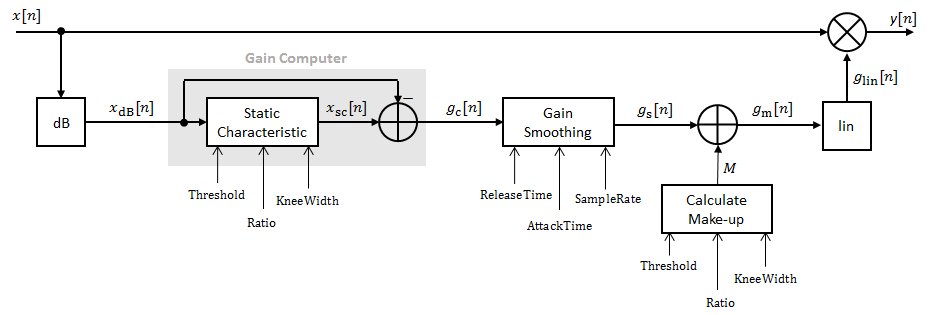
\includegraphics[width=200pt]{slike/kompresija.png}
    \centering
    \caption{Blok dijagram kompresora}
    \label{kompresija}
\end{figure}

Diskretizirani ulazni signal se pretvara u decibele radi intuitivnijih prikaza %(izbaciti ovo i početi od parametara?)
 operacija, a nakon kompresije se vraća u linearnu domenu. Glavni parametri kompresije su ~\cite{b3}:
 \begin{itemize}
   \item{prag (\textit{Treshold}) – razina ulaznog signala koja određuje početak kompresije,}
   \item{omjer kompresije (\textit{Ratio}) – omjer promjene signala na ulazu i izlazu,}
   \item{pojačanje (\textit{Make-up gain}) – pojačanje ukupne razine signala,}
   \item{vrijeme reakcije (\textit{Attack time}) – vrijeme koje je potrebno da kompresor počne djelovati na
   amplitudu signala prema definiranom omjeru kompresije nakon što signal prijeđe prag,}
   \item{vrijeme otpuštanja (\textit{Release time}) – vrijeme koje je potrebno da kompresor prestane djelovati na
   amplitudu signala i vrati se omjer kompresije 1:1 nakon što signal ponovno prijeđe prag,}
   \item{koljeno (\textit{Knee}) – prijelazno područje u izlaznoj karakteristici kompresora, %izlaznoj=prijenosnoj?
   mjesto dodira signala i linije praga.}
 \end{itemize}

 Manipulacija spomenutih parametara rezultira različitim oblicima zvuka. Promjena koljena određuje koliko će
 „glatko“ kompresor rezati signal. Promjena vremena reakcije i otpuštanja također djeluje na uglađenost zvuka.
 Što su parametri manji, to će kompresoru trebati manje vremena za početak djelovanja na amplitudu pa će signal
 zvučati dotjeranije. Najveće promjene zvuka događaju se mijenjanjem praga jer on određuje koliko će posla imati
 kompresor i koliko će „zamaskirati“ originalni signal. Za optimalne parametre prema ~\cite{b2}, dobije se vidljiva
 razlika u vremenskoj domeni, što je prikazano na slikama \ref{ulaz_vrijeme} i \ref{komp_vrijeme}.
 Primjećujemo smanjenu razliku između dijelova signala s najvišim i najnižim amplitudama.

% Ovim projektom napravljen je kod za usporedbu originalnog i komprimiranog signala u vremenskoj i
% frekvencijskoj domeni što je vidljivo na slici \ref{komp_vrijeme}.

\begin{figure}[H]
    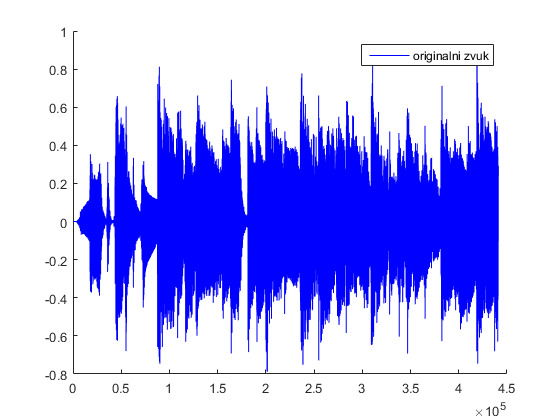
\includegraphics[width=200pt]{slike/def_orig.jpg}
    \centering
    \caption{Originalni signal u vremenskoj domeni}							%dodati legend u matlabu
    \label{ulaz_vrijeme}
\end{figure}

\begin{figure}[H]
    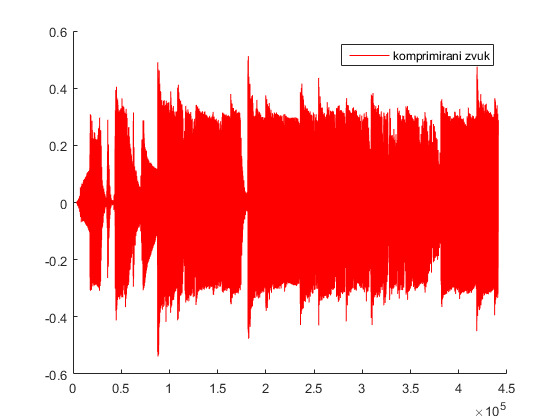
\includegraphics[width=200pt]{slike/def_kompr.jpg}
    \centering
    \caption{Komprimirani signal u vremenskoj domeni}							%dodati legend u matlabu
    \label{komp_vrijeme}
\end{figure}

% Na slici \ref{komp_spektar} vidljiva je razlika u spektru. Budući da se događaju promjene u amplitudi u
% vremenskoj domeni, to je u frekvencijskoj domeni vidljivo kao novonastala istosmjerna komponenta.
Na idućim slikama vidljiva je razlika u spektru. Budući da se događaju promjene u amplitudi u vremenskoj domeni,
to je u frekvencijskoj domeni vidljivo kao novonastala istosmjerna komponenta.

\begin{figure}[H]
    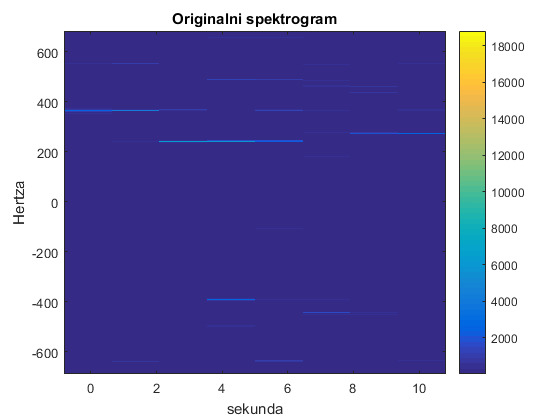
\includegraphics[width=200pt]{slike/originalni_spektrogram.jpg}
    \centering
    \caption{Spektrogram originalnog signala}
    \label{komp_ulaz_spektar}
\end{figure}

\begin{figure}[H]
    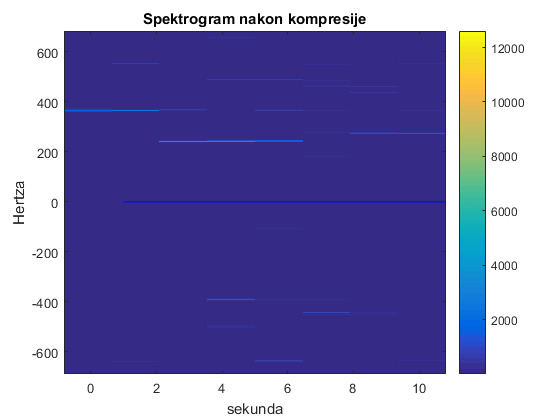
\includegraphics[width=200pt]{slike/spektrogram_nakon_kompresije.jpg}
    \centering
    \caption{Spektrogram komprimiranog signala}							%zasto DC komponenta??
    \label{komp_spektar}
\end{figure}

Kao što je već spomenuto, prekomjerna kompresija može utjecati na stvaranje zašumljenog, bezizražajnog
zvuka kao što je prikazano na slici \ref{komp_sum}. U ovom slučaju problem je prenizak prag.

\begin{figure}[H]
    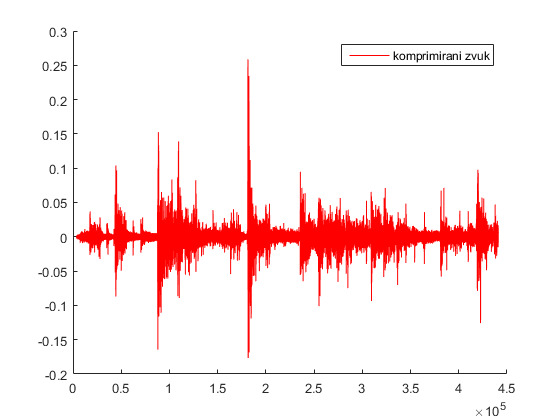
\includegraphics[width=200pt]{slike/prenizak_prag.jpg}
    \centering
    \caption{Vremenski prikaz komprimiranog signala uz prenizak prag}
    \label{komp_sum}
\end{figure}

U spektru je šum vidljiv kao nove spektralne komponente.

\section{DISTORZIJA}

Pojam distorzija odnosi se na izobličenje valnog oblika signala. Do distorzije može doći tijekom snimanja
ili reproduciranja zvuka, a u tom smislu radi se o neželjenim izobličenjima signala. Međutim, glazbenici
često unose različite vrste izobličenja kako bi dobili zanimljiviji zvuk. Najčešći oblik distorzije je
rezanje ulaznog signala nakon što amplituda prijeđe zadanu granicu (ograničavanje signala).
Rezanje signala (engl. clipping) je nelinearno izobličenje. Postoji mnogo načina rezanja signala a dvije
osnovne podjele su:

\begin{itemize}
  \item{Simetrična ili asimetrična karakteristika rezanja (izgled signala u vremenu prikazan je na slici
    \ref{dist_1})},
  \item{Oštri (engl. \textit{hard clipping}) ili zaobljeni (engl. \textit{soft clipping}) rubovi karakteristike
  rezanja (izgled signala u vremenu prikazan prikazan je na slici \ref{dist_2})}.
\end{itemize}

\begin{figure}[H]
    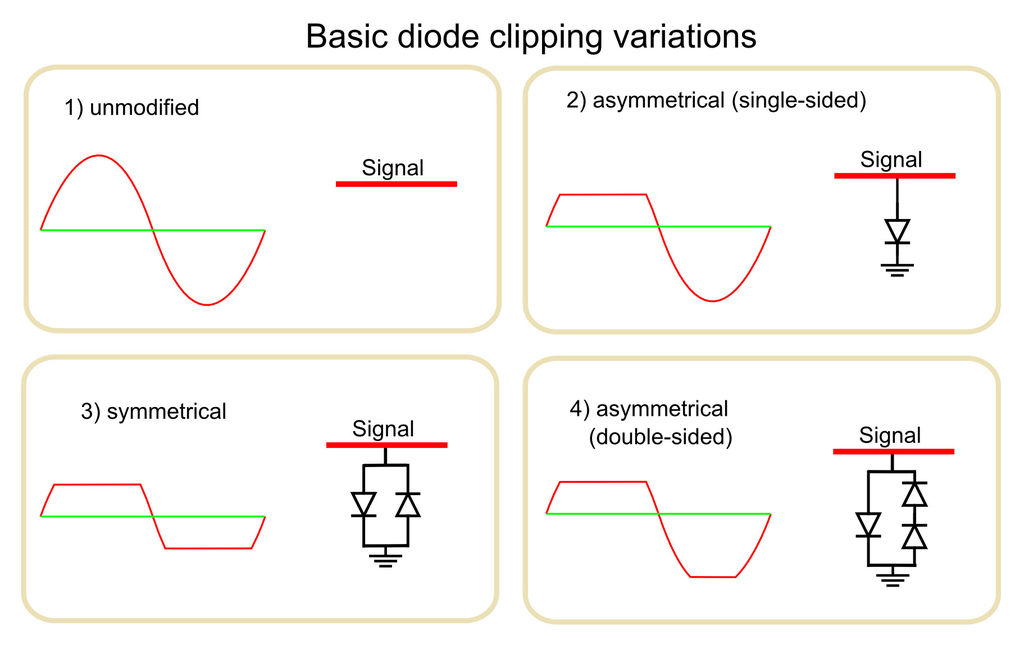
\includegraphics[width=200pt]{slike/dist_diode_clip.jpg}
    \centering
    \caption{Simetrično i antisimetrično rezanje signala}
    \label{dist_1}
\end{figure}

\begin{figure}[H]
    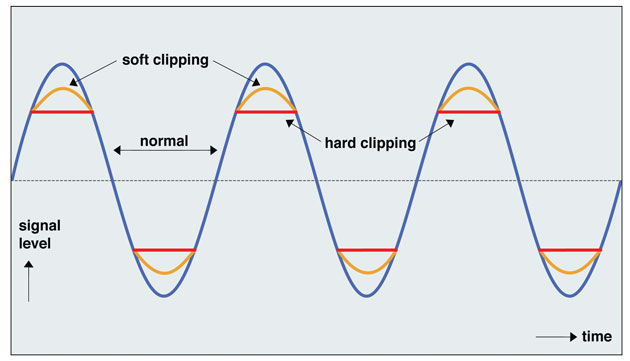
\includegraphics[width=200pt]{slike/dist_2.jpg}
    \centering
    \caption{\textit{Hard clipping} i \textit{soft clipping}}
    \label{dist_2}
\end{figure}

Spektar signala na kojeg je dodan efekt distorzije ovisi o funkciji po kojoj se mijenja ulazni signal. Ako je
funkcija parna, u spektru će se pojaviti parni harmonici, odnosno neparni harmonici ako je funkcija neparna.
U slučaju da funkcija nije niti parna niti neparna, izlazni signal sadržavat će i parne i neparne harmonike.
Ovakva vrsta distorzije naziva se harmonička distorzija. Harmonička distorzija vidljiva je u slučajevima kada
je na ulazu u sustav za distorziju signal samo sa jednom frekvencijskom komponentom. U stvarnosti je vrlo teško
snimiti zvuk samo jedne frekvencije, stoga spektar izlaznog signala ne sadrži samo parne ili neparne harmonijske
komponente. Ovakva vrsta distorzije naziva se intermodulacijska distorzija. Spektar izlaznog signala u ovom slučaju
sadržava frekvencije koje su jednake zbrojevima i razlikama frekvencija ulaznog signala.
\textit{Hard clipping} unosi neparne harmonike visokih amplituda zbog čega se na izlazu dobiva grubi zvuk.
Suprotno hard clippingu, \textit{soft clipping} unosi neparne harmonike manjih amplituda, stoga je zvuk na izlazu
manje grub i ugodniji za slušatelje.

U okviru ovog projekta realizirana su dva oblika distorzije: \textit{fuzz} efekt i \textit{overdrive} efekt.
\textit{Fuzz} je simetrično izobličenje s oštrim rubovima karakteristike rezanja ulaznog signala, a realiziran je
jednadžbom \ref{fuzz}.

\begin{equation}
  f(x)=\frac{x}{|x|}\*(1-e^{\frac{a\*x^2}{|x|}})
  \label{fuzz}
\end{equation}
Gdje je $x$ ulazni signal, a $a$ faktor kojim se definira razina distorzije.

Overdrive je simetrično izobličenje sa zaobljenim rubovima karakteristike rezanja ulaznog signala. Odabrana
funkcija za postizanje overdrive efekta definirana je jednadžbom \ref{overdrive}.

\begin{equation}
  f(x)=
    \begin{cases}
      2\*x, & 0 \leq |x|<\frac{1}{3} \\
      sgn(x)\cdot\frac{3-(2-3\*|x|)^2}{3}, & \frac{1}{3} \leq |x| < \frac{2}{3} \\
      sgn(x), & \frac{2}{3} \leq |x| \leq 1 \\
    \end{cases}
  \label{overdrive}
\end{equation}

Na slici \ref{A_original_spektar} prikazan je spektrogram originalnog zvuka, dok su na slikama
\ref{distorzija_fuzz} i \ref{distorzija_overdrive} prikazani spektrogrami nakon primjene \textit{fuzz} i
\textit{overdrive} efekta.

\begin{figure}[H]
    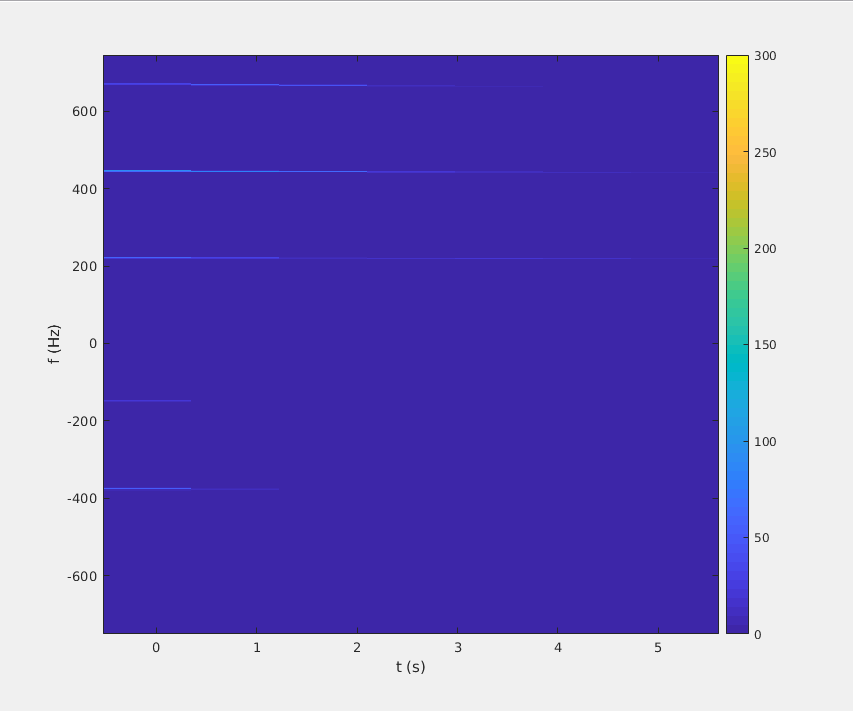
\includegraphics[width=200pt]{slike/A_ton.png}
    \centering
    \caption{Spektrogram originalnog signala (A ton)}
    \label{A_original_spektar}
\end{figure}

\begin{figure}[H]
    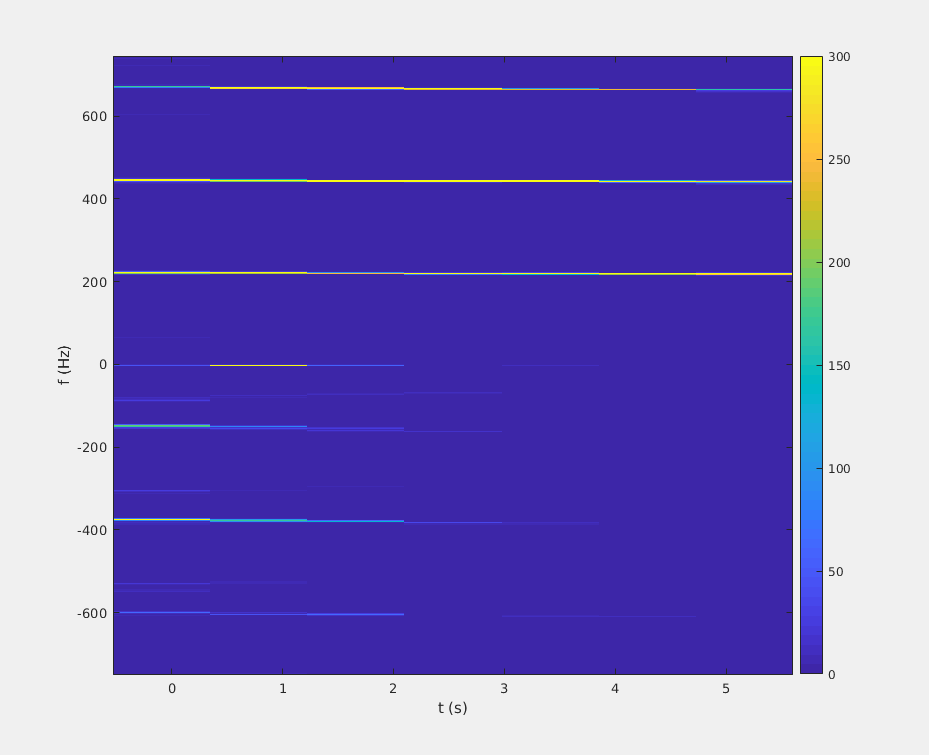
\includegraphics[width=200pt]{slike/distorzija_fuzz.png}
    \centering
    \caption{Spektrogram signala nakon primjene \textit{fuzz} efekta}
    \label{distorzija_fuzz}
\end{figure}

\begin{figure}[H]
    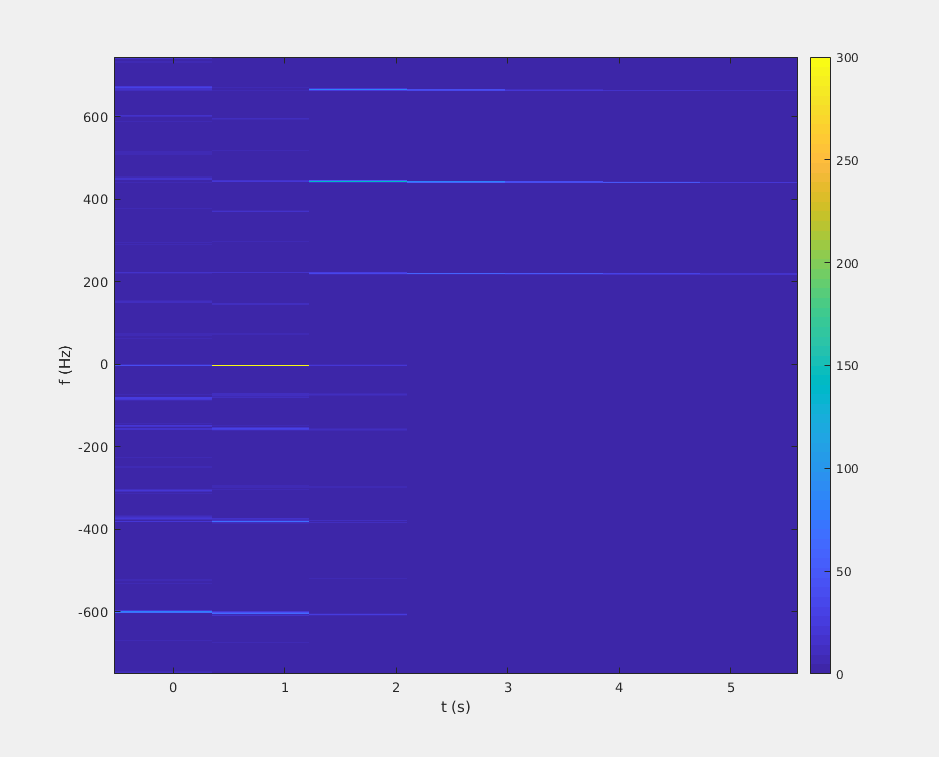
\includegraphics[width=200pt]{slike/distorzija_overdrive.png}
    \centering
    \caption{Spektrogram signala nakon primjene \textit{overdrive} efekta}
    \label{distorzija_overdrive}
\end{figure}

\section{\textit{FLANGER}}

\textit{Flanger} je zvučni efekt koji na ulazni signal unosi kašnjenje promijenjivog iznosa (najčešće manje
od 15 ms), te zakašnjeli signal dodaje na ulazni. Pritom se iznos kašnjenja mijenja kao sinusni signal
niske frekvencije - LFO (engl. \textit{Low Frequency Oscillator}, tipično 0.1 - 5 Hz)~\cite{b1}.
Primjena \textit{flanger} efekta svodi se, dakle, na dodavanje fazno moduliranog ulaznog signala na izvorni
signal. Na slici \ref{flang_simulink} prikazan je blok-dijagram FIR filtra kojim se realizira \textit{flanger}
efekt.

\begin{figure}[H]
    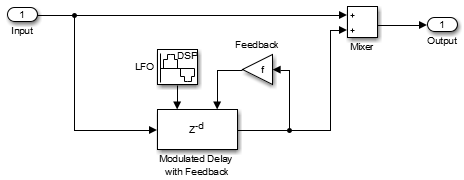
\includegraphics[width=200pt]{slike/flanger_simulink.png}
    \centering
    \caption{MATLAB model filtra za realizaciju \textit{flanger} efekta~\cite{b4}}
    \label{flang_simulink}
\end{figure}

FIR filtar koji se temelji na kašnjenju može se prikazati jednadžbom diferencija:
\begin{equation}
  y[n]=x[n]+g\*x[n-M]
  \label{flanger}
\end{equation}
gdje je $M$ promijenjivi iznos kašnjenja, a $g$ faktor kojim se pojačava ili atenuira zakašnjeli signal.
Budući da je iznos kašnjenja na izlazu iz LFO realan broj, prije modulacije potrebno je provesti zaokruživanje
na cijeli broj ili interpolaciju kojom se usrednjava vrijednost dvaju susjednih uzoraka.

Zvuk na koji je primijenjen \textit{flanger} prepoznatljiv je po efektu koji se popularno naziva
\textit{whooshing}. Taj se efekt javlja zbog konstruktivne i destruktivne interferencije između kombiniranih
zvučnih valova.

Slika \ref{flang_spektar} prikazuje spektrogram signala na koji je primijenjen \textit{flanger} uz LFO
frekvenciju 1 Hz, maksimalni iznos kašnjenja 5 ms te faktor pojačanja $g=0.7$. U odnosu na spektrogram originalnog
signala koji je prikazan slikom \ref{komp_ulaz_spektar}, vidljive su nove komponente koje su nastale uslijed
modulacije zakašnjelog ulaznog signala.

\begin{figure}[H]
    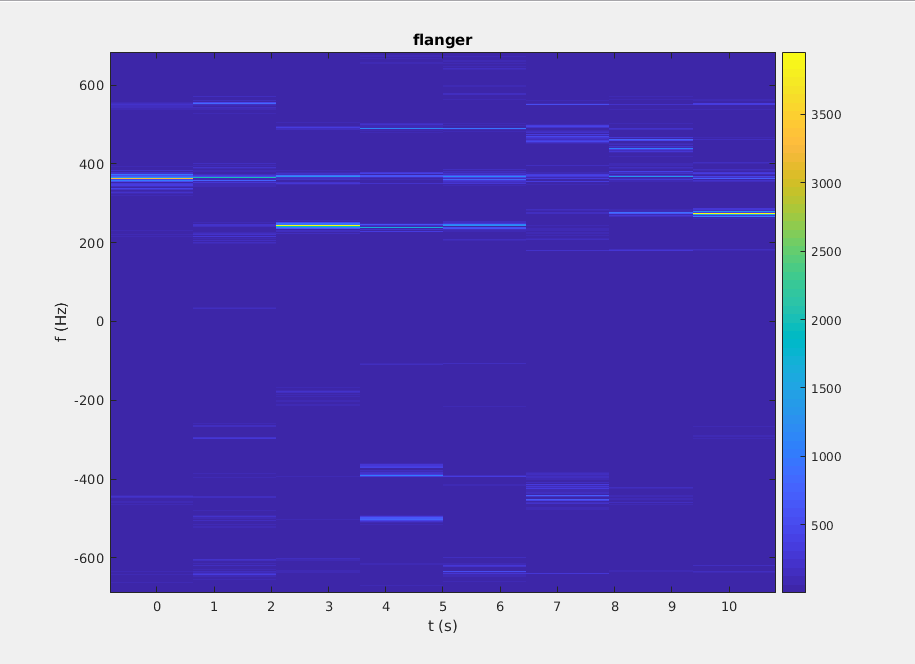
\includegraphics[width=200pt]{slike/flanger_spektar.png}
    \centering
    \caption{Spektrogram signala s \textit{flanger} efektom}
    \label{flang_spektar}
\end{figure}

\section{Odjek}

Efekt odjeka temelji se na efektu kašnjenja, koji se može opisati kao snimanje, odnosno otipkavanje, ulaznog signala
koji se zatim reproducira nakon određenog vremena. Signal kojemu je dodan efekt kašnjenja, može se
reproducirati više puta ili se ponovno snimiti što stvara ponavljajući zvuk. Osnovna struktura kašnjenja može
se ostvariti pomoću FIR ili IIR filtra ili kombinacijom dvaju filtara, gdje se efekt odjeka realizira pomoću
jednostavnog FIR filtra danog jednažbom (\ref{flanger}).
Gdje je:
\begin{equation}
  M = \tau/f_{s}
  \label{M}
\end{equation}

a $\tau$ i $f_{s}$:
 \begin{itemize}
   \item{$\tau$ - iznos kašnjenja signala,}
   \item{$f_{s}$ - frekvenciju otipkavanja.}
 \end{itemize}

Dodavanjem efekta odjeka na osnovni signal zvuk poprima dojam odbijanja zvuka od zida, dok se zapravo čuje
ponavljanje osnovnog signala. MATLAB model opisanog efekta dan je slikom \ref{echo_model}. Dodatni efekt povezan
s odjekom je efekt koji nastaje zbog povratne veze, a čuje se kao zvuk koji postepeno nestaje~\cite{b4}. Drugim riječima
vrijednost povratne veze određuje broj odjeka na način da neki postotak izlaza prosljeđuje na ulaz.
Model opisuje već danu jednadžbu FIR filtra uz dodatak povratne veze. Vrijednost $d$ u modelu odgovara vrijednosti
$M$ u jednadžbi filtra, a $f$ (\textit{FeedbackLevel}) pojačanje linije s dodanim efektom odjeka.

\begin{figure}[H]
    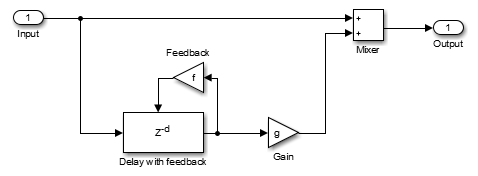
\includegraphics[width=200pt]{slike/echo_matlab.png}
    \centering
    \caption{MATLAB model odjeka}
    \label{echo_model}
\end{figure}

Na slici \ref{A_ton_vrijeme} prikazan je ulazni signal sviranja gitare u vremenu, a na slici \ref{echo_vrijeme}
prikazan je taj isti signal u vremenu na koji je dodan efekt odjeka. Ako se uspoređuju ulazni i obrađeni signal može se
primjetiti kako obrađeni signal izgleda "punije", odnosno vidi se kako je na ulazni signal superponiran dodatni signal.
Takvo ponašanje kod odjeka je očekivano zato što se obrađeni signal zbraja s ulaznim signalom. Na slici z dodanim
efektom odjeka može se vidjeti i da se jedno kratko vrijeme u početku ulazni i obrađeni signal podudaraju. Takav rezultat
je također očekivan jer efekt odjeka djeluje upravo tako da se ulaznom signalu superponira obrađeni signal nakon određenog
vremena kašnjenja.

\begin{figure}[H]
    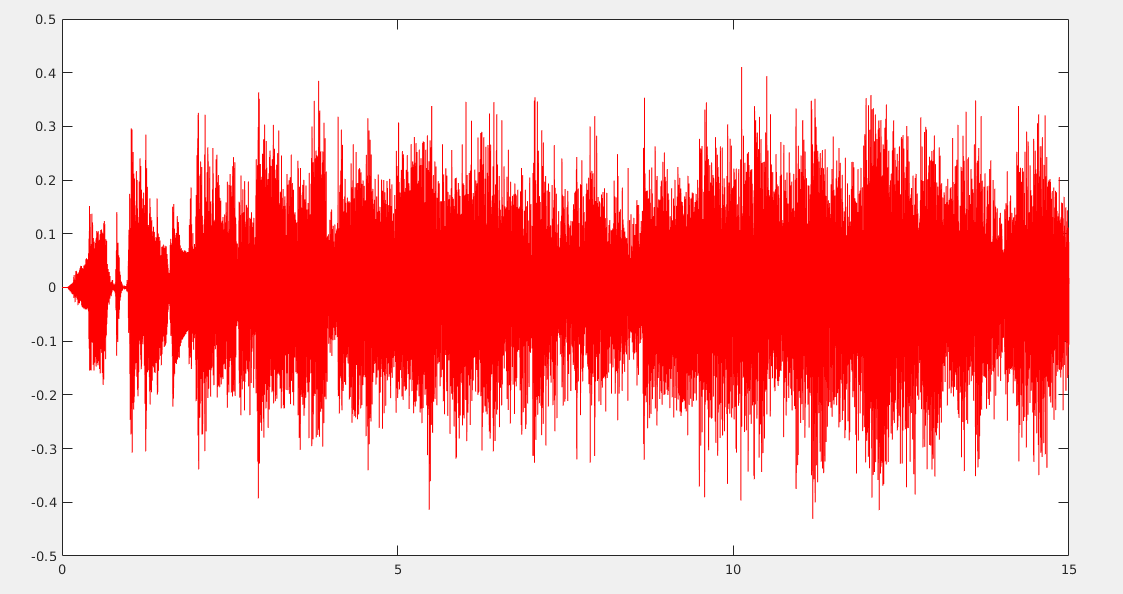
\includegraphics[width=200pt]{slike/echo_vrijeme.png}
    \centering
    \caption{Signal s dodanim odjekom u vremenu}
    \label{echo_vrijeme}
\end{figure}

Na slici \ref{A_original_spektar} prikazan je spektrogram A tona, dok je na slici \ref{echo} prikazan spektrogram
A tona s dodanim odjekom. Kad se uspoređuju spektrogrami ulaznog i obrađenog signala može se zaključiti da se
na spektrogramu vide frekvencijske komponente koje se na spektrogramu originalnog signala ne vide. Novonastale
frekvencijske komponente su u spektrogramu postavljene kao da se nadovezuju na originalni signal. Takav rezultat je
očekivan jer odjek na osnovni signal dodaje obrađeni ulazni signal te ga superponira ulaznom signalu nakon određenog
vremena kašnjenja. Spektrogram opisuje upravo takvo ponašanje.

\begin{figure}[H]
  \centerline{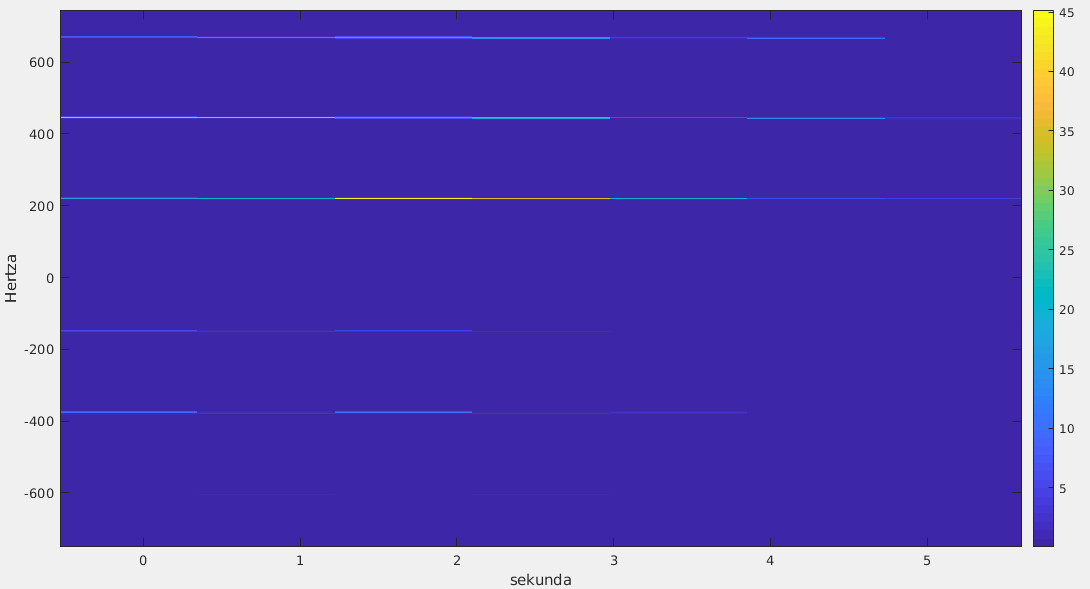
\includegraphics[width=200pt]{slike/A_ton_echo.png}}
  \caption{Spektrogram A tona s odjekom}
  \label{echo}
\end{figure}

Matematički model u MATLABu proveden je sa sljedećim vrijednostima parametara:
\begin{itemize}
  \item{$g$=1,}
  \item{$M$=$\tau$/$f_{s}$, gdje je $\tau$ zadan kao 1s, a $f_{s}$ zadana frekvencija otipkavanja: 48000Hz i}
  \item{pojačanje povratne veze $f$=0.5}
\end{itemize}

Podešavanjem parametra $g$ dobijemo bolje ili lošije vidljive novonastale frekvencijske komponente u
spektrogramu, gdje je maksimalna vrijednost parametra 1. Kako se vrijednost navedenog parametra povećava, na spektrogramu se bolje uočava ponavljanje
osnovnog tona. Na grafu obrađenog signala u vremenskoj domeni sa što većom vrijednošću parametra $g$ jasnije
se vidi na kojoj sekundi je osnovnom signalu nadodan odjek. Drugim riječima, iz grafa obrađenog signala u vremenskoj domeni
može se lakše odrediti zadano vrijeme kašnjenja. Određivanje vremena kašnjenja ovisi i o parametru $\tau$ koji
utječe na signal na način da što je $\tau$ manji, graf obrađenog signala je sličniji ulaznom signalu. Takvo ponašanje
u vremenskoj domeni se preslikava na ponašanje koje čitamo iz spektrograma.
Pojačanje povratne veze $f$ na vremensku domenu utječe na način da što je parametar veće vrijednosti, u prikazu
obrađenog signala bolje se raspoznaje koliko puta signal odjekne. Što bi taj parametar bio manji, na prikazu obrađenog
signala bi se moglo raspoznati manje odjeka. Utjecaj parametra na spektrogram je analogan utjecaju parametra na vremensku
domenu, odnosno što je parametar veći, na spektrogramu su bolje vidljive novonastale frekvencijske komponente.
Razlike signala u vremenskoj domeni s različitim vrijednostima parametara vidljive su slikom \ref{A_usporedba}, dok je
ulazni signal A tona prikazan slikom \ref{A_ton_vrijeme}.

\begin{figure}[H]
  \centerline{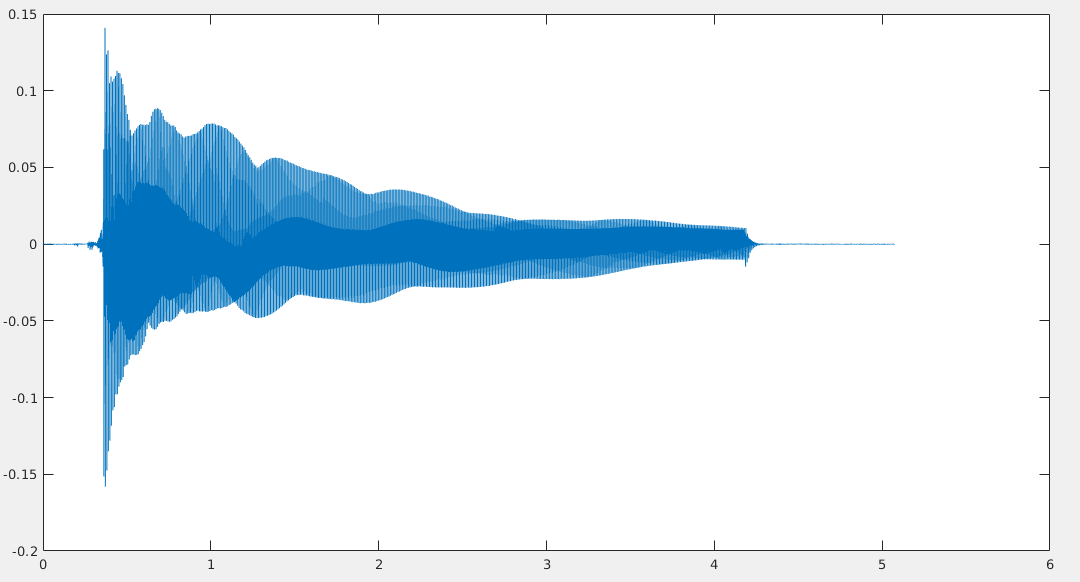
\includegraphics[width=200pt]{slike/A_ton_vrijeme.png}}
  \caption{A ton u vremenskoj domeni}
  \label{A_ton_vrijeme}
\end{figure}

\begin{figure}[H]
  \centerline{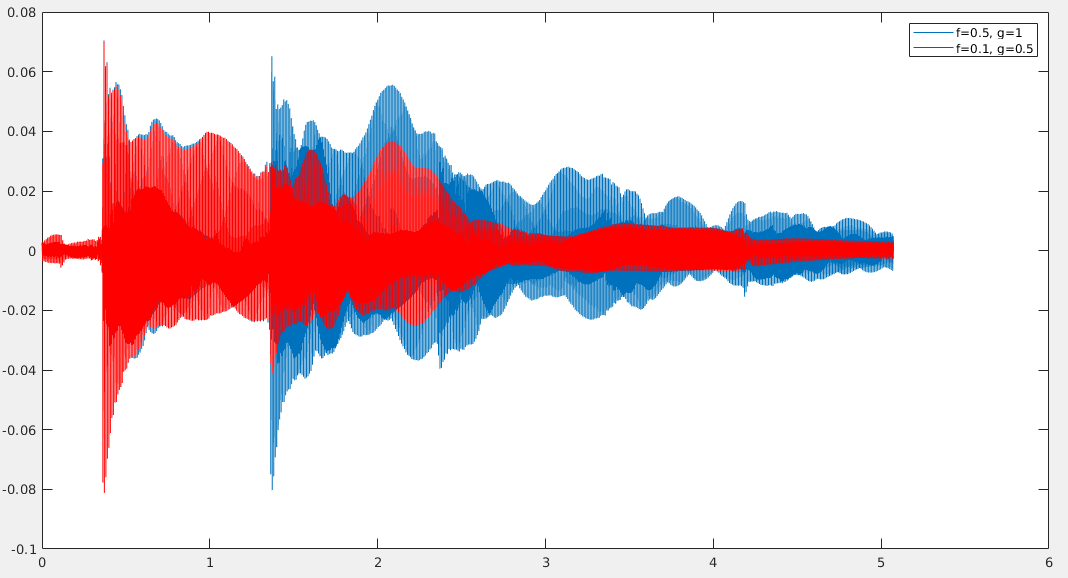
\includegraphics[width=200pt]{slike/A_ton_usporedba.png}}
  \caption{Usporedba prikaza obrađenog A tona}
  \label{A_usporedba}
\end{figure}

Plavi signal na slici \ref{A_usporedba} odgovara obrađenom signalu
s već navedenim vrijednostima parametara, a crveni signal odgovara obrađenom signalu s vrijednostima parametara
$f$=0.1 i $g$=0.5.


\section{Tremolo}
Tremolo je efekt koji se dobiva amplitudnom modulacijom tonova niskom frekvencijom (nekoliko Hz). Ta pojava se čuje
kao drhtanje. Često se ovaj efekt miješa sa vibratom, ali vibrato se dobiva modulacijom visine tona (pitch-modulation).

Općenito, modulacija je postupak u kojemu se u prijenosni signal utiskuje signal informacije. Amplitudna modulacija
se postiže promjenom amplitude modulacijskog signala. Prijenosni signal služi za prijenos informacije, ali on ne
sadrži informaciju. Modulacijski signal sadrži informaciju, odnosno on je sam po sebi informacija. Postupak ampliudne
 modulacije prikazan je slikom \ref{amp_mod}.

 \begin{figure}[H]
   \centerline{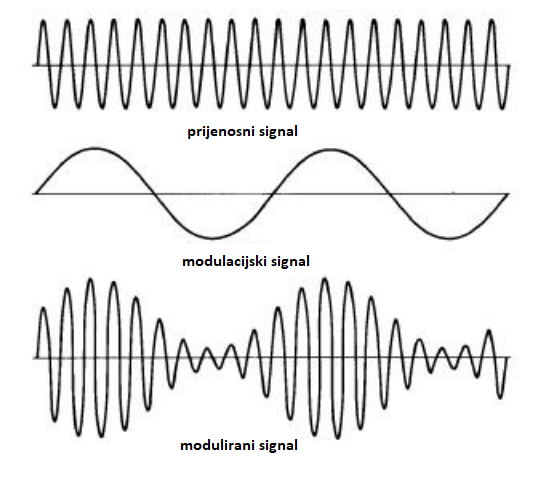
\includegraphics[height=200pt]{slike/amplitudna_modulacija.png}}
   \caption{Amplitudna modulacija}
   \label{amp_mod}
 \end{figure}

 Prijenosni signal je matematički zapisan kao:
\begin{equation}
  u_{p} = U_{pm}\*sin(\omega_{p}\*t+\Phi_{0})
  \label{mat_zapis}
\end{equation}

Modulacijski:
\begin{equation}
  u_{m} = U_{mm}\*sin(\omega_{m}\*t)
  \label{mod_zapis}
\end{equation}

Pri čemu je: $\omega_{p}$=2$\omega_{m}$, odnosno $f_{p}$>>$f_{m}$.
Važan parametar modulacije je dubina ili indeks modulacije. Indeks modulacije je omjer između najveće promjene
amplitude modulacijskog signala i najveće promjene amplitude prijenosnog signala. Formula za indeks modulacije je:
\begin{equation}
  m_{a} = U_{mm}/U_{pm},
  \label{indeks_mod}
\end{equation}
gdje je: $U_{mm}$  amplituda modulacijskog signala, a $U_{pm}$ amplituda prijenosnog signala.
U ovom projektu, tremolo je izveden u programu MATLAB. Amplitudna modulacije je izračunata na temelju sljedećeg izraza:
\begin{equation}
  y(n) = (1+ m_{a}\*m(n))\*x(n),
  \label{matlab_mod}
\end{equation}
gdje su:
\begin{itemize}
  \item{$x(n)$ zvučni signal (u ovom slučaju zvuk gitare),}
  \item{$m(n)$ modulacijski signal niske frekvencije do 20 Hz,}
  \item{$m_{a}$ je indeks modulacije ( za $m_{a}$=1 je modulacija maksimalna, a za $m_{a}$=0 ne dolazi do modulacije)}
\end{itemize}

Budući da su i zvučni i modulacijski signal sinusni sa frekvencijama $f_{c}$ i $f_{x}$, nakon primjene ovoga efekta, pojavit
će se nove komponente oko frekvencije $f_{c}$ i to na frekvencijama $f_{c}$-$f_{x}$ i $f_{c}$+$f_{x}$. Dodatne komponente
dobro se vide na
spektrogramu koji je prikazan na slici \ref{tremolo_izlaz} u odnosu na spektrogram ulaznog spektrograma prikazanog
slikom \ref{tremolo_ulaz}. Komponente su se pojavile na očekivanim frekvencijama oko frekvencije osnovnog
signala.

\begin{figure}[H]
   \centerline{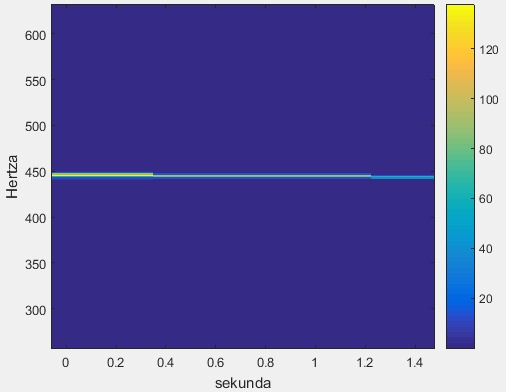
\includegraphics[height=200pt]{slike/tremolo_ulaz.jpeg}}
   \caption{Spektrogram A tona}
   \label{tremolo_ulaz}
 \end{figure}

 \begin{figure}[H]
   \centerline{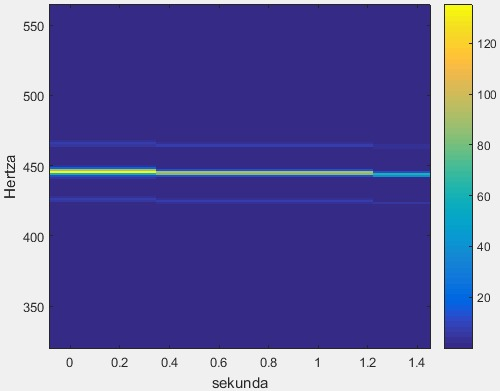
\includegraphics[height=200pt]{slike/tremolo_izlaz.jpeg}}
   \caption{Spektrogram A tona nakon primjene tremolo efekta}
   \label{tremolo_izlaz}
 \end{figure}

\section{Zaključak}
Digitalna obradba signala sastavni je dio glazbene produkcije. Zvučni efekti, često nastali kao
posljedica slučajnih pogrešaka u sviranju i obradbi signala, glavni su faktori u manipulaciji zvukom.

Kompresija smanjuje dinamički raspon signala bez distorzije, bez potrebe za rezanjem
(\textit{clippingom}).

\begin{thebibliography}{00}
\bibitem{b1} Cardiff University, ``Digital Audio Effects'',
	\url{www.cs.cf.ac.uk/Dave/CM0268/PDF/10_CM0268_Audio_FX.pdf}
  \bibitem{b2} Compressor - MATLAB,
  \url{https://www.mathworks.com/help/audio/ref/compressor.html}
  \bibitem{b3} ``Dinamička obrada audiosignala'',
  \url{https://www.fer.unizg.hr/_download/repository/EAT13_Dinamicka_obrada_audio_signala_2017-18.pdf}
  \bibitem{b4} Delay-Based Effects - MATLAB,
  \url{https://www.mathworks.com/help/audio/examples/delay-based-audio-effects.html}
  \bibitem{b5} Effects Explained: Echo, Delay, and Reverb
  \url{http://www.gibson.com/News-Lifestyle/Features/en-us/effects-explained-echo-delay.aspx}
\end{thebibliography}

\end{document}
